\chapter{Evaluation}
\label{chap:evaluation}

We evaluate different parity update schemes through our CodFS prototype. We
deploy CodFS on a testbed with 22 nodes of commodity hardware configurations.
Each node is a Linux machine running Ubuntu Server 12.04.2 with kernel version
3.5. The MDS and OSD nodes are each equipped with Intel Core i5-3570 3.4GHz
CPU, 8GB RAM and two Seagate
ST1000DM003 7200RPM 1TB SATA harddisk. For each OSD, the first harddisk is used
as the OS disk while the entire second disk is used for storing chunks. The
client nodes are equipped with Intel Core 2 Duo 6420 2.13GHz CPU, 2GB RAM and a
Seagate ST3160815AS 7200RPM 160GB SATA harddisk. Each node has a Gigabit
Ethernet card installed and all nodes are connected via a Gigabit full-duplex
switch.

\section{Baseline Performance}
\label{sec:evaluation_baseline}

\begin{figure}[!t]
\centering
 \begin{subfigure}{0.48\linewidth}
     \includegraphics[width=\linewidth]{charts/transfer/eps/up/rdp_6}
     \caption{Sequential write}
     \label{fig:rdp_write}
 \end{subfigure}
 \hspace{0.005\linewidth}
 \begin{subfigure}{0.48\linewidth}
     \includegraphics[width=\linewidth]{charts/transfer/eps/up/rs_6}
     \caption{RS write}
     \label{fig:rs_write}
 \end{subfigure}
 \begin{subfigure}{0.48\linewidth}
     \includegraphics[width=\linewidth]{charts/transfer/eps/down/rdp_6}
     \caption{Sequential read}
     \label{fig:rdp_read}
 \end{subfigure}
 \hspace{0.005\linewidth}
 \begin{subfigure}{0.48\linewidth}
     \includegraphics[width=\linewidth]{charts/transfer/eps/down/rs_6}
     \caption{RS read}
     \label{fig:rs_read}
 \end{subfigure}
 \caption{Aggregate read/write throughput of CodFS using the RDP code with
	 $(n,k)=(6,4)$.}
 \label{fig:data}
% \vspace{-5pt}
\end{figure}


We derive the achievable aggregate read/write throughput of CodFS and analyze
its best possible performance.  Suppose that the encoding overhead can be
entirely masked by our parallel design.  If our CodFS prototype can
effectively mitigate encoding overhead and evenly distribute the operations
among OSDs, then it should achieve the theoretical throughput. 

We define the notation as follows.  Let $M$ be the total number of OSDs in the
system, and let $B_{in}$ and $B_{out}$ be the available inbound and outbound
bandwidths (in network or disk) of each OSD, respectively.  Each encoding scheme
can be described by the parameters $n$ and $k$, following the same definitions
in \S\ref{sec:ec_background}.  
%To encode a segment, we divide it into $k$ chunks of the same size and encode
%the $k$ chunks into $n$ chunks, such that any $k$ out of $n$ chunks can be used
%to reconstruct the original segment. 

We derive the effective aggregate write throughput (denoted by
$T_{write}$).  Each primary OSD, after encoding a segment, stores one chunk
locally and distributes $n-1$ chunks to other secondary OSDs.  This introduces
an additional $(n-1)/k$ times of segment traffic among the OSDs.
Similarly, for the effective aggregate read throughput (denoted by
$T_{read}$), each primary OSD collects $(k-1)$ chunks for each read segment
from the secondary OSDs. It introduces an additional $(k-1)/k$ times of segment
traffic.  Thus, $T_{write}$ and $T_{read}$ are given by: 

\vspace{-5pt}
\begin{equation*}
    T_{write} = \frac{M\times B_{in}}{1+\frac{n-1}{k}} , \hspace{20pt}
    T_{read} = \frac {M\times B_{out}}{1+\frac{k-1}{k}}.
\end{equation*}

%\begin{equation}
%    T_{write} = \frac{M B_{in}}{1+\frac{n-1}{k}}
%\end{equation}
%\begin{equation}
%    T_{read} = \frac {M B_{out}}{1+\frac{k-1}{k}}
%\end{equation}

We evaluate the aggregate read/write throughput of CodFS, and compare the
experimental results with our theoretical results.  We first conduct
measurements on our testbed and find that the effective disk and network
bandwidths of each node are 144MB/s and 114.5MB/s, respectively.  Thus,
the nodes are network-bound, and we set $B_{in}\!=\!B_{out}\!=$ 114.5MB/s in
our model.  We configure CodFS with one node as the MDS and $M$ nodes as OSDs,
where $6\!\le\!M\!\le\!10$.  We consider the RAID-6 Reed-Solomon (RS)
\cite{reed60} and RDP
code \cite{corbett04} with $(n,k) = (6,4)$.  The coded chunks are distributed
over the $M$ OSDs.  We
have 10 other nodes in the testbed as clients that transfer streams of
segments simultaneously. 

Figure~\ref{fig:data} shows the aggregate read/write throughput of CodFS
versus the number of OSDs for different segment sizes from 8MB to 64MB. We see
that the throughput results match closely with the theoretical results, and the
throughput scales linearly with the number of OSDs.  For example, when $M=10$
OSDs are used, CodFS achieves read and write throughput of at least 580MB/s
and 450MB/s, respectively.  

We observe that both RDP and RS codes have almost identical throughput, although
RS codes have higher encoding overhead \cite{plank09}.  The reason is that CodFS
masks the encoding overhead through parallelization. 

\section{Evaluation on Synthetic Workload}
\label{eval:synthetic}

\begin{figure}[t]
\centering
 \begin{subfigure}[t]{0.48\linewidth}
     \includegraphics[width=\linewidth]{charts/seq_write/eps/seq_write}
     \caption{Sequential write}
	 \label{fig:seq_write}
 \end{subfigure}
 \begin{subfigure}[t]{0.48\linewidth}
     \includegraphics[width=\linewidth]{charts/rand_write/eps/rand_write}
     \caption{Random write}
	 \label{fig:rand_write}
 \end{subfigure}
 \begin{subfigure}[t]{0.48\linewidth}
     \includegraphics[width=\linewidth]{charts/seq_read/eps/seq_read}
     \caption{Sequential read}
	 \label{fig:seq_read}
 \end{subfigure}
 \begin{subfigure}[t]{0.48\linewidth}
     \includegraphics[width=\linewidth]{charts/recovery/eps/recovery}
     \caption{Recovery}
	 \label{fig:recovery}
 \end{subfigure}
 \caption{Throughput of CodFS under different update schemes.}
 \label{fig:update_schemes}
\end{figure}

We now evaluate the four delta-based parity update schemes (i.e., \FO, \FL, 
\PL, and \PLR) using our CodFS prototype under a synthetic workload.  Unless
otherwise stated, we use the RDP code \cite{corbett04} with $(n,k) = (6,4)$,
16MB segment size, and the same cluster configuration as in
\S\ref{sec:evaluation_baseline}.  We measure the sequential write, random
write, sequential read, and recovery performance of CodFS using IOzone
\cite{iozone}. For \PLR, we use the baseline approach described in
\S\ref{sec:reserve_strategies} and fix the size of reserved space to 4MB,
which is equal to the chunk size in our configuration. We trigger a merge
operation to reclaim the reserved space when it becomes full.
%We will evaluate other strategies and discuss the impact of merging in
%\S\ref{sec:reserve_evaluation}.  
Before running each test, we format the chunk partition of each OSD to
%clear all previous fragmentation and to 
restore the OSD to a clean state, and drop the buffer cache in all OSDs to
ensure that any difference in performance is attributed to the update schemes.

We note that an update to a data chunk in RDP \cite{corbett04} involves more
updates to parity chunks than in RS codes (see \cite{plank13} for illustration),
and hence generates larger-size parity deltas.  This triggers more frequent
merge operations as the reserved space becomes full faster. 

\subsection{Sequential Write Performance}
\label{eval:seq_write}

Figure~\ref{fig:seq_write} shows the aggregate sequential write throughput of
CodFS under different update schemes, in which all clients simultaneously
write 2GB of segments to the storage cluster.  As expected, there is only
negligible difference in sequential write throughput among the four update
schemes as the experiment only writes new data.

\subsection{Random Write Performance}
\label{eval:rand_write}

We use IOzone to simulate intensive small updates, in which we issue uniform
random writes with 128KB record length to all segments uploaded in
\S\ref{eval:seq_write}.  In total, we generate 16MB of updates for each
segment, which is four times of the reserved space size in \PLR.  Thus, $\PLR$
performs at least four merge operations per parity chunk (more merges are
needed if the coding scheme triggers the updates of multiple parts of a parity
chunk for each data update). 
Figure~\ref{fig:rand_write} shows the numbers of I/Os per second (IOPS) 
of the four update schemes.  Results show that \FO performs the worst among
the four, with at least $21.0\%$ fewer IOPS than the other three schemes. This
indicates that updating both the data and parity chunks in-place incurs extra
disk seeks and parity read overhead, thereby significantly degrading update
efficiency.  The other three schemes give similar update performance with less
than ${4.1}\%$ difference in IOPS.

%we observe negligible impact on the average performance between \PL and
%\PLR.}
%As both \PL and \PLR update data chunks in-place, we can argue that the poor
%performance of the \FO scheme is mainly due to in-place parity updates. Here,
%\FL, \PL, and \PLR all use a logging-based approach towards parity
%deltas. During an update, the \FO scheme is the only scheme in this case
%that requires reading the old parity chunk for performing update with the
%parity delta.
%
%One reason for such behaviour can be explained by properties of inline erasure
%coding. During an update, the OSDs need to read old data chunks for computing
%the parity delta. Since reading an old chunk requires a disk seek no matter
%what update scheme is used, this inevitable cost takes away most advantages of
%using a log-based approach for data chunks. 
%
%It is also worth pointing that the \PLR scheme only suffers a slight penalty
%($\red{<6.8}\%$) for placing the parity deltas in the reserve space. 

%\paragraph{Level of Disk Fragmentation.} 

\subsection{Sequential Read Performance} 
\label{eval:seq_read} 

Sequential read and recovery performance are affected by disk fragmentation in data and parity
chunks.  To measure fragmentation, we define a metric $F_{avg}$ as the 
\textit{average number of non-contiguous fragments per chunk} that are read
from disk to rebuild the up-to-date chunk.  Empirically, $F_{avg}$ is found by
reading the physical block addresses of each chunk in the underlying file
system of the OSDs using the \texttt{filefrag -v} command which is available
in the \texttt{e2fsprogs} utility. For each chunk, we obtain the number of
non-contiguous fragments by analyzing its list of physical block addresses and
lengths.  We then take the average over the chunks in all OSDs. 
%An average value is calculated by dividing the total number of non-contiguous
%fragments by the total number of chunks in all OSDs.

%Although modern disk drives use read-ahead caches and perform request
%reordering to reduce the overall number of seeks \cite{shriver98}, we use
%$F_{avg}$ to give an approximation on the number of disk seeks each OSD needs
%to perform to read each chunk. Besides the number of disk seeks, a higher
%$F_{avg}$ also implies a larger merging overhead.  However, we will be able
%to isolate such overhead when we compare recovery throughput between the \PLR
%scheme and the \FO scheme.  

\begin{table}[t]
  \centering
        \begin{tabular}{ccrrrr}
        \toprule
        & & FO    & FL    & PL    & PLR \\ \hline
        \multirow{2}[0]{*}{Synthetic} & Data  & 0     & 29.41 & 0     & 0 \\ \vspace{-1.1pt}
              & Parity & 0     & 117.66 & 117.66 & 0 \\ 
        \bottomrule
        \end{tabular}%
        \caption{Average non-contiguous fragments per chunk 
            ($F_{avg}$) after random writes for synthetic workload.}
  \label{table:synthetic_fragmentation}%
\end{table}%

Table~\ref{table:synthetic_fragmentation} shows the value of $F_{avg}$
measured after random writes in \S\ref{eval:rand_write}.  Both \FO and \PLR have $F_{avg} = 0$
%do not produce any non-contiguous fragments on disk 
as they either store updates and deltas in-place or in a contiguous space next
to their parity chunks.  \FL is the only scheme that contains
non-contiguous fragments for data chunks, and it has $F_{avg} = 29.41$ in the
synthetic benchmark. 
%Roughly speaking, the disk has to seek $29.41$ times to rebuild a data chunk
%in \FL under the synthetic benchmark. 
Logging parity deltas introduces higher level of disk fragmentation. On
average, both \FL and \PL produce $117.66$ non-contiguous fragments per parity
chunk in the synthetic benchmark. We see that $F_{avg}$ of parity chunks is
about $4\times$ that of data chunks. This conforms to our RDP configuration
with $(n,k)=(6,4)$ since each segment consists of four data chunks and modifying
each of them once will introduce a total of four parity deltas to each parity
chunk. 

Figure~\ref{fig:seq_read} shows a scenario which we execute a sequential read
after intensive random writes. We measure the aggregate sequential read
throughput under different update schemes.  In this experiment, all clients
simultaneously read the segments after performing the updates described in
\S\ref{eval:rand_write}.

Since CodFS only reads data chunks when there are no node failures, no
performance difference in sequential read is observed for \FO, \PL and \PLR.
However,  the sequential read performance of \FL drops by half when
compared with the other three schemes. This degradation is due to the combined
effect of disk seeking and merging overhead for data chunk updates. The result
also agrees with the measured level of disk fragmentation shown in
Table~\ref{table:synthetic_fragmentation} where \FL is the only scheme that
contains non-contiguous fragments for data chunks.

\subsection{Recovery Performance}
\label{eval:recovery}

%Another reason is that logging parity updates has a
%higher impact on the level of disk fragmentation than logging data updates, which
%we will address below. 

We evaluate the recovery performance of CodFS under a double failure scenario,
and compare the results among different update schemes. We trigger the recovery
procedure by sending \texttt{SIGKILL} to the CodFS process in two of the OSDs.
We measure the time between sending the kill signal and receiving the
acknowledgement from the MDS reporting all data from the failed OSDs
are reconstructed and redistributed among the available OSDs.

Figure~\ref{fig:recovery} shows the measured recovery throughput for different update
schemes. \FO is the fastest in recovery and achieves substantial difference in
recovery throughput (up to ${4.5\times}$) compared with \FL due to the
latter suffering from merging and disk seeking overhead for both data and
parity chunks. By keeping data chunks updates in-place, \PL achieves a modest
increase in recovery throughput compared with \FL.  We also see the benefits
of \PLR for keeping delta updates next to their parity chunks.  \PLR
gains a ${3\times}$ improvement on average in recovery throughput when
compared with \PL.

\subsection{Reserved Space versus Update Efficiency}
\label{eval:reserve_comparison}

We thus far evaluate the parity update schemes under the same coding
parameters $(n,k)$.  Since \PLR trades storage space for update efficiency, we
also compare $\PLR$ with other schemes that use the reserved space for
storage.  Here, we set the reserved space size to be equal to the chunk size
in \PLR with $(n,k) = (6,4)$.  This implies that a size of two extra chunks is
reserved per segment.   For \FO, \FL, and \PL, we substitute the reserved
space with either two data chunks or two parity chunks.  We realize the
substitutions with erasure coding using two coding parameters: $(n,k) = (8,6)$
and $(n,k) = (8,4)$, which in essence store two additional data chunks, and
two additional parity chunks over $(n,k) = (6,4)$, respectively.  Since RDP
requires $n-k=2$, we choose the Cauchy RS code \cite{blomer95} as the coding
scheme.  We also fix the chunk size to be 4MB, so we ensure that each coded
segment in all 7 configurations takes 32MB of storage including data, parity,
and reserved space.  

Figure~\ref{fig:reserve_comparison} shows the performance of random writes 
and recovery under the same synthetic workload described in
\S\ref{eval:rand_write}.  Results show that the $(8,4)$
schemes perform significantly worse than the $(8,6)$ schemes in random writes,
since having more parity chunks implies more parity updates.  Also, we
see that \FO $(8,6)$ is slower than \PLR $(6,4)$ by at least $20\%$ in terms
of IOPS, indicating that allocating more data chunks does not necessarily
boost update performance. Results of recovery agree with those in
\S\ref{eval:recovery}, i.e., both \FO and \PLR give significantly higher
recovery throughput than \FL and \PL. 

\begin{figure}[!t]
\centering
\begin{tabular}{c@{\ }c}
\includegraphics[width=0.48\linewidth]{charts/reserve_overhead/eps/reserve_overhead_randw} & 
\includegraphics[width=0.48\linewidth]{charts/reserve_overhead/eps/reserve_overhead_recover}
\vspace{-3pt}\\
\mbox{\small (a) Random write} &
\mbox{\small (b) Recovery}
\end{tabular}
\vspace{-3pt}
\caption{Throughput comparison under the same storage
 overhead using Cauchy RS codes with various $(n,k)$.}
\label{fig:reserve_comparison}
\vspace{-6pt}
\end{figure}

\subsection{Summary of Results}

We make the following observations from our synthetic evaluation.
First, although our configuration has twice as many data chunks as
parity chunks, updating data chunks in-place in \PL does not help much in
recovery throughput.  This implies that the time spent on reading and
rebuilding parity chunks dominates the recovery performance.  Second, as shown
in Table~\ref{table:synthetic_fragmentation}, both \FO and \PLR do not
produce disk seeks. Thus, we can attribute the difference in recovery
throughput between \FO and \PLR solely to the merging overhead for parity
updates. We see that \PLR incurs less than ${9.2\%}$ in recovery
throughput on average compared with \FO. We regard this as a reasonable
trade-off since recovery itself is a less common operation than random writes.
%\PLR provides efficient update performance as \FL, while maintaining a
%comparable recovery throughput to \FO.

\section{Evaluation on Real-world Traces}
\label{eval:trace}

Next, we evaluate CodFS by replaying the MSR Cambridge and Harvard NFS traces
analyzed in \S\ref{sec:trace}.

\subsubsection {MSR Cambridge Traces}
%\begin{table}[t] \footnotesize
%  \centering
%        \begin{tabular}{ccrrrr}
%        \toprule
%        &  & FO    & FL    & PL    & PLR \\ \hline
%        \multirow{2}[0]{*}{src22} & Data  & 0     & 0.73  & 0     & 0 \\ \vspace{2.5pt}
%              & Parity & 0     & 2.82  & 2.83  & 0 \\ 
%        \multirow{2}[0]{*}{mds0} & Data  & 0     & 16.24 & 0     & 0 \\ \vspace{2.5pt}
%              & Parity & 0     & 64.90 & 64.87 & 0 \\ 
%        \multirow{2}[0]{*}{rsrch0} & Data  & 0     & 9.63  & 0     & 0 \\ \vspace{2.5pt}
%              & Parity & 0     & 38.46 & 38.43 & 0 \\ 
%        \multirow{2}[0]{*}{usr0} & Data  & 0     & 9.78  & 0     & 0 \\ \vspace{2.5pt}
%              & Parity & 0     & 39.07 & 39.08 & 0 \\ 
%        \multirow{2}[0]{*}{web0} & Data  & 0     & 9.98  & 0     & 0 \\ \vspace{2.5pt}
%              & Parity & 0     & 39.87 & 39.84 & 0 \\ 
%        \multirow{2}[0]{*}{ts0} & Data  & 0     & 18.65 & 0     & 0 \\ \vspace{2.5pt}
%              & Parity & 0     & 74.55 & 74.59 & 0 \\ 
%        \multirow{2}[0]{*}{stg0} & Data  & 0     & 27.18 & 0     & 0 \\ \vspace{2.5pt}
%              & Parity & 0     & 108.67 & 108.63 & 0 \\ 
%        \multirow{2}[0]{*}{hm0} & Data  & 0     & 36.03 & 0     & 0 \\ \vspace{2.5pt}
%              & Parity & 0     & 144.06 & 143.84 & 0 \\ 
%        \multirow{2}[0]{*}{prn1} & Data  & 0     & 3.51  & 0     & 0 \\ \vspace{2.5pt}
%              & Parity & 0     & 14.01 & 13.99 & 0 \\ 
%        \multirow{2}[0]{*}{proj0} & Data  & 0     & 45.66 & 0     & 0 \\ \vspace{-1.1pt}
%              & Parity & 0     & 182.60 & 182.04 & 0 \\ 
%        \bottomrule
%        \end{tabular}%
%        \caption{Average non-contiguous fragments per chunk 
%            ($F_{avg}$) after replaying different MSR Cambridge traces.}
%  \label{table:msr_fragmentation}%
%\end{table}%

%\begin{figure}[t]
%    \centering
%    \includegraphics[width=\linewidth]{charts/msr_frag/eps/msr_frag}
%    \vspace{-12pt}
%        \caption{Average non-contiguous fragments per chunk 
%            ($F_{avg}$) after replaying different MSR Cambridge traces.}
%    \label{fig:msr_fragmentation}
%\end{figure}

To limit the experiment duration, we choose 10 of the 36 volumes for
evaluating the update and recovery performance. We choose the traces with the
number of write requests between $800,000$ and $4,000,000$. Also, to
demonstrate that our design does not confine to a specific workload, the
traces we select for evaluation all come from different types of servers.

%by removing all read requests.  Skipping read
%requests shortens the experiment without having any effect in the update and
%recovery performance. Second, we 
We first pre-process the traces as follows.
%compacting the address space. We remove chunks that are not accessed
%throughout the entire trace period.  
We adjust the offset of each request accordingly so that the offset maps to
the correct location of a chunk.  We ensure that the locality of requests
to the chunks is preserved. 
%For example, two write requests to chunk $x$ and chunk $y$ in the trace will
%never be assigned to the same chunk in the compacted trace. Finally, 
If there are consecutive requests made to a sequence of blocks, they will be
combined into one request to preserve the sequential property during replay.

We configure CodFS to use $10$ OSDs and split the trace evenly to
distribute replay workload among $10$ clients. We first write the segments
that cover the whole working set size of the trace.  Each client then replays
the trace by writing to the corresponding offset of the preallocated segments.
We use RDP \cite{corbett04} with $(n,k)=(6,4)$ and 16MB segment size. 

\subsection{Update Performance.} Figure~\ref{fig:msr_update} shows the aggregate
number of writes replayed per second. To perform a stress test, we ignore the
original timestamps in the traces and replay the operations as fast as possible.
First, we observe that
traces with a smaller coverage (as indicated by the percentage of updated WSS in
Table~\ref{table:msr}) in general results in higher IOPS no matter which update
scheme is used. For example, the \texttt{usr0} trace with $13.08\%$ updated
WSS shows more than ${3\times}$ update performance when compared with the
\texttt{src22} trace with $99.57\%$ updated WSS.  This
is due to a more effective client LRU cache when the updates are focused on a
small set of chunks. The cache performs write coalescing and reduces the number
of round-trips between clients and OSDs. Second, we see that the four schemes
exhibit similar behaviour across traces. \FL, \PL and \PLR show comparable
update performance.  This leads us to the same implication as in
\S\ref{eval:rand_write} that the dominant factor influencing update performance
is the overhead in parity updates. Therefore, the three schemes that use a
log-based design for parity chunks all perform significantly better than \FO. On
average, \PLR is ${63.1}\%$ faster than \FO.

\begin{figure}[t]
    \centering
    \includegraphics[width=\linewidth]{charts/msr_update/eps/msr_update}
    \vspace{-12pt}
    \caption{Number of write operations per second replaying the selected MSR
        Cambridge traces under different update schemes.}
    \label{fig:msr_update}
\end{figure}

\begin{figure}[t]
    \centering
    \includegraphics[width=\linewidth]{charts/msr_recovery/eps/msr_recovery}
    \vspace{-12pt}
    \caption{Recovery throughput in a double failure scenario after replaying
        the selected MSR Cambridge traces under different update schemes.}
    \label{fig:msr_recovery}
\end{figure}

\subsection{Recovery Performance.} Figure~\ref{fig:msr_recovery} shows the
recovery throughput in a two-node failure scenario. We see that in all traces,
\FL and \PL are slower than \FO and \PLR in recovery.   Also, \PLR outperforms
\FL and \PL more significantly in traces where there is a large number of
writes and $F_{avg}$ is high.  For example, the measured $F_{avg}$ for the
\texttt{proj0} trace is $45.66$ and $182.6$ for data and parity chunks, 
respectively, and \PLR achieves a remarkable ${10\times}$ speedup in recovery
throughput over \FL.  On the other hand, \PLR performs the worst in the
\texttt{src22} trace, where $F_{avg}$ is only $0.73$ and $2.82$ for data and
parity chunks, respectively.  Nevertheless, it still manages to give an
${11.7}\%$ speedup over \FL.

\subsection{Evaluation of Reserved Space}
\label{eval:reserve_evaluation}

We evaluate our workload-aware approach in managing the
reserved space size (see \S\ref{sec:reserve_strategies}). We use the Harvard
NFS traces, whose 41-day span provides long enough duration to examine the
effectiveness of shrinking, merging, and prediction.
We calculate the \textit{reserved space storage overhead} using the following
equation, which is defined as the additional storage space allocated by the
reserved space compared with the original working set size without any reserved
space:
%
\begin{equation*} \label{eq:overhead} \Gamma = \frac{\sum Reserved Space
        Size}{\sum (Data Size + Parity Size)}.
\end{equation*}
%
A low $\Gamma$ means that the reserved space is small
compared with the total size of all data and parity chunks. 

%As we set the reserved space size to be multiples of chunk size to avoid
%creating unusable holes during shrinking, we obtain the lower bound of
%$\Gamma$ for an $(n,k)$ erasure code by setting the reserved space size to be
%equal to the chunk size.}
%

%\begin{equation*} \label{eq:lower_bound}
%    \Omega(\Gamma) = \frac{(n-k)(ChunkSize)}{n(ChunkSize)} = \frac{n-k}{n} .
%\end{equation*}


Using the above metric, we evaluate our workload-aware framework used in \PLR
by simulating the Harvard NFS traces. We set the segment size to 16MB and
use the Cauchy RS code \cite{blomer95} with $(n,k)=(10,8)$. 
%\del{The lower bound of $\Gamma$ is given by $(6-4)/6=0.33$.} 
Here, we compare our workload-aware approach with three baseline approaches,
in which we fix the reserved space size to 2MB, 8MB, and 16MB without
any adjustment.

We consider two variants of our workload-aware approach. The
\textit{shrink+merge} approach executes the shrinking operation at 00:00 and
12:00 on each day, followed by a merge operation on each chunk. The
\textit{shrink only} approach is identical to the \textit{shrink+merge}
approach in shrinking, but does not perform any merge operation after
shrinking (i.e., it does not free the space occupied by the parity deltas).
On the first day, we initialize the reserved space to 16MB.  We follow the
framework described in \S\ref{sec:reserve_strategies} and set the smoothing
factor $\alpha = 0.3$.
%Here, we first obtain the utility of each parity chunk's reserved space
%($u^t_p$) using Equation~\ref{eq:utility_now} with the smoothing factor
%$\alpha=0.05$. We then perform shrinking using the shrink size ($c^*_p$)
%calculated by Equation~\ref{eq:shrink_size}.  Finally, the size of reserved
%space for new parity chunks on the next day ($P_{t+1}$) is determined by
%Equation~\ref{eq:predict} using the smoothing factor $\beta=0.05$. 

%\paragraph{Shrink with Merge.} This strategy is identical in setting as the
%shrink strategy. However, we invoke a merge operation that combines all parity
%deltas  after shrinking the
%reserved space of each parity chunk.

\subsubsection{Simulation Results} 

Figure~\ref{fig:harvard_ratio} shows the value
of $\Gamma$ under the three different approaches by simulating the 41-day
Harvard traces.  The 2MB, 8MB, and 16MB baseline approaches give 
$\Gamma=0.2$, $0.8$, and $1.6$, respectively, throughout the entire trace
since they never shrink the reserved space.  The values of $\Gamma$ for both
workload-aware variants drop quickly in the first week of trace and then
gradually stabilize.  At the end of the trace, the \textit{shrink only}
approach has $\Gamma$ of about $0.36$.  With merging, the
\textit{shrink+merge} approach further reduces $\Gamma$ to $0.12$. $\Gamma$ is
lower than that of the 2MB baseline, as around $13\%$ of parity chunks end up
with zero reserved space size.

Aggressive shrinking may increase the number of merge
operations. We examine such an impact by showing the average number of merges
per $1000$ writes in Figure~\ref{fig:harvard_merge}. A lower value implies lower
write latency since fewer writes are stalled by merge operations.  We make a
few key observations from this figure. First, the 16MB baseline gives the
best results among all strategies, since it keeps the largest reserved space
than other baselines and workload-aware approaches throughout the whole
period. On the contrary, using a fixed reserve space that is too small
increases the number of merges significantly. This effect is shown by the 2MB
baseline. Second, the performance of the workload-aware approaches matches
closely with the 8MB and 16MB baseline approaches most of the time.  Day 30-40
is an exception in which the two workload-aware approaches perform
significantly more merges than the 16MB baseline approach. This reflects
the penalty of inaccurate prediction when the reserved space is not large
enough to handle the sudden bursts in updates.  Third, although the
\textit{shrink+merge} approach has a lower reserved space storage overhead, it
incurs more penalty than the \textit{shrink only} approach in case of a
misprediction. However, we observe that on average less than $1\%$ of writes
are stalled by a merge operation regardless of which approach is used (recall
that the merge is performed every $1000$ writes).  Thus, we expect that there
is very little impact of merging on the performance in \PLR.

%However, we see that the shrink strategy 
%shrinking introduces more merge operations on some days. This
%reflects the penalty of inaccurate prediction and excessive shrinking as the reserved
%space is not large enough to store all the updates. But in most cases, the
%shrink strategy has similar number of merge operations to the baseline
%strategy. Also, the number of merge operations is far reduced in the shrink with
%merge strategy due to the periodical merge which free up reserved space.
%In a nutshell, compared with the daily number of updates for each segment,
%the average number of merge for all three strategies are small. Since 
%less than $number of merge/number of updates\%$ updates needs merge operation,
%which is fairly small so that the update performance is guaranteed. However,
%using deallocation significantly reduced the storage overhead. The deallocation
%with merge strategy perform best in both evaluation but it introduces the
%overhead of active merge operations. 

\begin{figure}[t!]
    \centering
    \includegraphics[width=\linewidth]{charts/harvard_ratio/harvard_ratio.eps}
    \vspace{-2em}
    \caption{Reserved space overhead under different shrink strategies in the Harvard
        trace.}
    \label{fig:harvard_ratio}
\end{figure}


\begin{figure}[t!]
    \centering
    \includegraphics[width=\linewidth]{charts/harvard_merge/harvard_merge.eps}
    \vspace{-2em}
    \caption{Average number of merges per 1000 writes under different shrink
        strategies in the Harvard trace.}
    \label{fig:harvard_merge}
\end{figure}

%\subsection{Discussion}
%
%Our experiments show that CodFS can effectively mask the coding overhead by
%comparing the read/write throughput with a theoretical model. Results from both
%synthetic workload and the MSR Cambridge traces evaluation show that \PLR
%is as good as \FL and \PL in updates. In recovery, 
%\PLRis only slightly worse than \FO. To summarize, our design
%achieves update efficiency without compromising recovery performance. 

\subsection{Summary of Results}

We show that \PLR achieves efficient updates and recovery.  It significantly
improves the update throughput of \FO and the recovery throughput of \FL. 
We also evaluate our workload-aware approach on reserved space management. 
We show that the \textit{shrink+merge} approach can reduce the reserved space
storage overhead by more than half compared to the 16MB baseline approach, with
slight merging penalty to reclaim space.  
%Here, we only propose a simple
%heuristic for reserved space management.  We pose the design of more advanced
%algorithms as future work.
